\subsection{Audiogestaltung und Inspiration}
Das Konzept der Installation beruht auf einem klassischen Step-Sequenzer. Solche Sequenzer steuern die Klangerzeugung eines Synthesizers dahingehend, dass sowohl Rhythmus als auch Tonhöhe programmiert werden können. Der Name bezieht sich dabei auf die einzelnen „Steps“ die mit Tönen belegt werden können. Klassische analoge Step-Sequenzer wie der Roland TB 303 bieten 16 Schritte an, womit also pro Durchlauf 16 Töne gespielt werden können. Somit entspricht jeder Schritt einer 16tel Note eines Taktes. Es ist hervorzuheben, dass bei einem Step-Sequenzer die Noteneingabe nicht unmittelbar zu einer Klangerzeugung führt. Stattdessen tastet ein Impuls nacheinander alle „Steps“ ab und übermittelt die Daten an den Klangerzeuger. Nachdem der Impuls einmal durchgelaufen ist, beginnt der er wieder bei dem ersten Step. Dadurch entstehen repetitive Tonfolgen, sogenannte Loops. Step-Sequenzer haben gerade aufgrund dieser Beschränkung zahlreiche Genre wie Acid House, Electronic Body Music und Drum and Bass entscheidend geprägt.

Das Konzept der Installation weicht in mehreren Punkten vom klassischen Step-Sequenzer ab. Zum Einen gibt es statt 16 Schritten nur 8. Außerdem ist die Tonauswahl auf 5 Tonhöhen pro Schritt begrenzt. Des Weiteren wird ist ein Ton nur so lange aktiviert, wie auch eine Person auf dem entsprechenden Feld steht. Das musikalische Konzept berücksichtigt diese Einschränkungen. Da nur 5 Töne gespielt werden können und auch nur 8 Steps zur Verfügung stehen, wird ein Backing Track benötigt, der eine harmonische Grundlage für das Spiel des Instrumentes bietet.

Anspruch der Installation war es aber weniger ein komplexes Instrument zu bieten, viel mehr eine musikalische Spielwiese. Aus diesem Grund liegt die Entscheidung nahe, sich die technischen Beschränkungen zu Nutze zu machen. Es wurde also auf eine Skala zurückgegriffen, die einerseits nur 5 Töne hat und andererseits keine Halbtonschritte aufweist: die Anhemitonische Pentatonik. Der Vorteil liegt darin, dass keine kleinen Sekunden und Tritoni gespielt werden können, die für unsere Hörgewohnheiten „unrein“ klingen. Durch diese Maßnahme wurde also sichergestellt, dass unabhängig von Menge und Position der Benutzer ein recht harmonisches Gesamtbild entsteht, auch wenn dadurch auf die Leittonwirkung einer Diatonik oder Hemitonischen Pentatonik verzichtet werden muss. Außerdem war der Tonumfang natürlich auf eine Oktave beschränkt, mehr als 5 Tonhöhen hätten das musikalische Ergebnis interessanter gestaltet aber auch die Nutzerfreundlichkeit eingeschränkt. Da die Installation in erster Linie intuitiv bedienbar sein sollte, wurde der Tonumfang nicht weiter ausgebaut.

Für den experimentellen Modus der Installation wurden drei Backing Tracks mit jeweils 5 zugehörigen Tonhöhen vorproduziert. Der durchlaufende Impuls wurde auf die Geschwindigkeit des entsprechenden Backing Tracks angepasst und die zugehörigen Töne auf die Felder gemappt. Da der Klangerzeuger kein Synthesizer sondern ein Sampler war, mussten die Einzeltöne im Voraus synthetisiert und gerendert werden. Grundsätzlich wurden eher sphärische Klänge mit langem Nachhall (entweder Reverb oder Hüllkurvengenerator) eingesetzt, da die Benutzer der Installation keinen Einfluss auf die Länge des Tons hatten. In Hüllkurvenparametern gesprochen musste also der Attack deutlich hörbar sein um ein auditives Feedback zu geben, die Sustainlautstärke musste relativ schnell erreicht werden und wesentlich leiser als der Attack sein, damit sich bei mehreren Personen die Sounds nicht zu stark überdeckten. Dadurch wurden relativ perkussive Klänge erzeugt, die durch den Nachhall eine gewisse Stetigkeit erreichten. Die Backing Tracks bildeten das rhythmische und harmonische Grundgerüst und wurden ebenfalls im Voraus produziert und gerendert. Dabei wurde Wert darauf gelegt, zwar eine harmonische Orientierung zu bieten, der Backing Track sollte jedoch keine komplexe harmonische Struktur aufweisen. In den Backing Tracks wurde also ebenfalls weitgehend auf die oben erwähnte Pentatonik zurückgegriffen, um aber ein wenig musikalische Spannung zu kreieren, wurden an ausgewählten Stellen auch Töne aus diatonischen Skalen verwendet.

Für den Challenge Modus wurden ebenfalls drei Backing Tracks und passende Töne vorproduziert, da jedoch die technischen und konzeptionellen Bedingungen andere waren, soll darauf noch näher eingegangen werden. Das Ziel des Challenge Modus ist es, mit der Installation bekannte Lieder nachzuspielen, ähnlich wie bei Guitar Hero. Problematisch ist jedoch, dass die Reaktionsgeschwindigkeit der Benutzer nicht so schnell ist wie es eigentlich nötig wäre. Das größte Hindernis ist jedoch, dass die Nutzer die Installation verlassen müssen, wenn sie keinen Ton spielen wollen. Sobald sie auf irgendeinem Feld stehen und der Impuls dieses erreicht wird der Ton getriggert, auch wenn er falsch ist. Anders gesagt: Die Zustände der Nutzer auf dem Spielfeld sind analog, benötigt wären aber digitale Zustände, an oder aus. Aus diesem Grund mussten Songs gefunden werden, die einerseits recht bekannt sind, ein minimales Tonspektrum aufweisen und langsam genug sind um mit der Installation spielbar zu sein. Die Entscheidung fiel auf „Smoke on the water“ von Deep Purple, „Paint it black“ von den Rolling Stones und “One” von Swedish House Mafia.

Die Ausschnitte der Lieder die benutzt werden sollten, wurden zunächst nachgespielt und aufgenommen. Dabei war es wichtig, hervorstechende Klangeigenschaften der Originale zu berücksichtigen um den Wiedererkennungswert nicht zu verlieren. Bei „Smoke on the water“ wurde beispielsweise ein bekannter britischer Röhrenverstärker mit vorgeschaltetem Overdrive verwendet. Nachdem alle Einzelspuren aufgenommen waren musste bestimmt werden, welche Spuren den Backing Track bildeten und welche Spur von den Nutzern gespielt werden sollte. Der Backing Track wurde dann ohne die entsprechende Spur gerendert. Die Spur die der Nutzer spielen sollte, musste nun in kleine Samples geschnitten werden um auf die verschiedenen Felder aufgeteilt werden zu können.

\begin{figure}[htbp] 
  \centering
     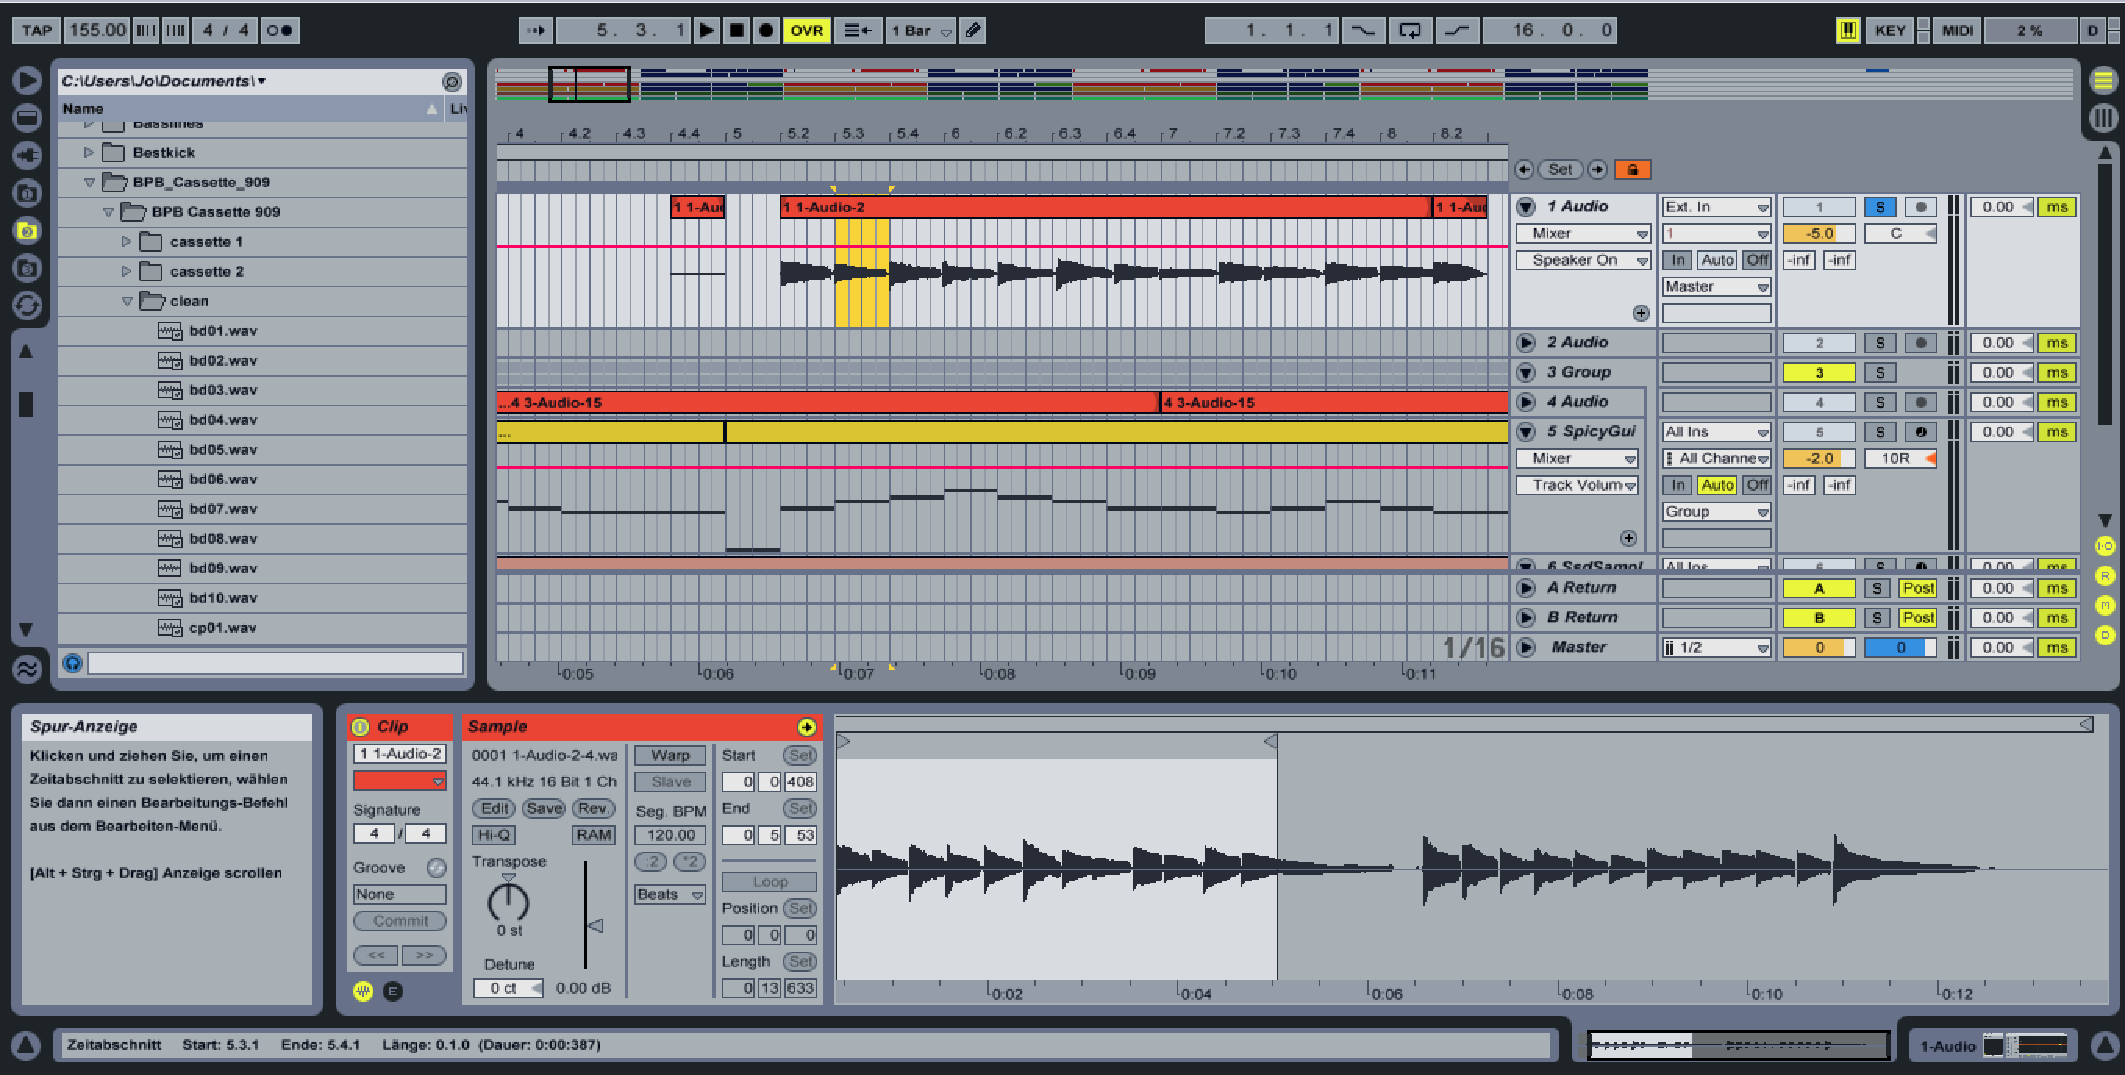
\includegraphics[width=0.9\textwidth]{images/Musikkonzeption}
  \caption{Schneiden der Spuren in Ableton Live}
  \label{fig:audio1}
\end{figure}

Dabei ergaben sich in einigen Fällen Probleme bezüglich der Tonlänge. Da die Schritte des Step-Sequenzers immer auf einen bestimmten Rhythmuswert quantisiert waren, zum Beispiel 8tel oder 16tel Noten, mussten hinsichtlich Synkopen oft Kompromisse eingegangen werden. Bei „One“ führte dies dazu, dass der Impuls so schnell war, dass das Lied damit praktisch unspielbar wurde. Für den Challenge Modus erwies sich damit das Konzept der Soundmatrix insgesamt als relativ ungeeignet, während im experimentellen Modus musikalisch interessante Ergebnisse erreicht wurden.